%%%%%%%%%%%%%%%%%%%%%%%%%%%%%%%%%%%%%%%%%%%%%%%%%%%%%%%%%%%%%%%%%%%%%%%%%%%%%%%%
%%%%%%%%%%%%%%%%%%%%%%%%%%%%%%%%%%%%%%%%%%%%%%%%%%%%%%%%%%%%%%%%%%%%%%%%%%%%%%%%
\subsection{Motivation}

The proposed method's motivation lies in the simple but powerful fact that is,
in general, exhibited through figure \ref{fig:face}: Assume a pose estimate
residing in a neighbourhood of a 2D LIDAR sensor's pose within a given map;
then the value of the CAER metric between the scan measured by the sensor and
the map-scan captured from the estimate within the map is simultaneously
proportional to both the estimate's location error and orientation error.
Formally the proposed method's foundations rest on Observation
\ref{obs:observation_o}:

%%%%%%%%%%%%%%%%%%%%%%%%%%%%%%%%%%%%%%%%%%%%%%%%%%%%%%%%%%%%%%%%%%%%%%%%%%%%%%%%
\begin{customobs}{O}
  \label{obs:observation_o} It may be observed that there are conditions such
  that Hypothesis \ref{hpt:hypothesis_h} stands true.
\end{customobs}

%%%%%%%%%%%%%%%%%%%%%%%%%%%%%%%%%%%%%%%%%%%%%%%%%%%%%%%%%%%%%%%%%%%%%%%%%%%%%%%%
\begin{customhpt}{H}
  \label{hpt:hypothesis_h}
  There exists $\hat{\bm{p}} \in  \mathbb{R}^2 \times [-\pi,+\pi)$ such that
  $\hat{\bm{p}} \in \mathcal{V}: \|\bm{p}-\hat{\bm{p}}\|_2 \leq \delta \leq \delta_0$
  is an admissible pose estimate solution to Problem \ref{prob:the_problem}
  (Def. \ref{def:definition_7}), where set $\mathcal{V}$ and $\delta_0$ are
  defined by Conjecture
  \ref{cnj:conjecture_c}.
\end{customhpt}

%%%%%%%%%%%%%%%%%%%%%%%%%%%%%%%%%%%%%%%%%%%%%%%%%%%%%%%%%%%%%%%%%%%%%%%%%%%%%%%%
\begin{customcnj}{C}
  \label{cnj:conjecture_c}
  Let the unknown pose of a 2D range sensor measuring range scan $\mathcal{S}_R$
  (Def. \ref{def:definition_1}) be $\bm{p}(x,y,\theta)$ with respect to the
  reference frame of map $\bm{M}$.
  Let $\mathcal{H}$ be a set of pose hypotheses within the free (i.e.
  traversable) space of $\bm{M}$:
  $\mathcal{H} = \{\hat{\bm{p}}_i(\hat{x}_i,\hat{y}_i,\hat{\theta}_i)\} \subseteq \texttt{free}(\bm{M})$,
  $i \in \texttt{I} = \langle 0,1,\dots,|\mathcal{H}|-1\rangle$.
  Let $f_{\psi}^{\bm{M}}$ be the $\psi$-field on $\bm{M}$
  (Def. \ref{def:definition_4}) such that $f_{\psi}^{\bm{M}}(\mathcal{H})= \Psi$.
  Let the field's locational and orientational densities be
  $d_{\bm{l}}$ and $d_{\alpha}$.
  Let $\hat{\bm{p}}_\omega \in \mathcal{H}$ and $\psi_0,\delta_0 \in \mathbb{R}_{>0}$
  such that $f_{\psi}^{\bm{M}}(\hat{\bm{p}}_\omega ) = \psi_0$ and
  $\|\bm{p}-\hat{\bm{p}}_j\|_2 \leq \delta_0$ for all
  $\hat{\bm{p}}_j \in \mathcal{H}: f_{\psi}^{\bm{M}}(\hat{\bm{p}}_j) \leq \psi_0$.
  Let now $\mathcal{V} = \{\hat{\bm{p}}_i \in \mathcal{H}: f_{\psi}^{\bm{M}}(\hat{\bm{p}}_i) \leq \psi_0,
  \|\bm{p}-\hat{\bm{p}}_i\|_2 \leq \delta_0\}$.
  Without loss of generality there exist $d_{\bm{l}}, d_{\alpha}$, and
  $\psi_0,\delta_0$ such that for all
  $\hat{\bm{p}}_\mathcal{V} \in \mathcal{V}$:
  \begin{align}
    f_{\psi}^{\bm{M}}(\hat{\bm{p}}_\mathcal{V}) < f_{\psi}^{\bm{M}}(\hat{\bm{p}}) \ \ \Leftrightarrow \ \
    \|\bm{p}-\hat{\bm{p}}_\mathcal{V}\|_2 < \|\bm{p}-\hat{\bm{p}}_{}\|_2 \nonumber
  \end{align}
  for any $\hat{\bm{p}}_{} \in \mathcal{X} = \mathcal{H} \setminus  \mathcal{V}: \|\bm{p}-\hat{\bm{p}}_{}\|_2 > \delta_0$.
\end{customcnj}

%%%%%%%%%%%%%%%%%%%%%%%%%%%%%%%%%%%%%%%%%%%%%%%%%%%%%%%%%%%%%%%%%%%%%%%%%%%%%%%%
\begin{remark}
  \label{rem:remark_1}
  The composition of
  $\mathcal{H} = \mathcal{V} \cup \mathcal{X} \cup \mathcal{W}$, where
  $\mathcal{W} = \hat{\bm{p}} \in {\mathcal{H} \setminus \mathcal{V}}: \|\bm{p}-\hat{\bm{p}}\|_2 \leq \delta_0$.
  With regard to the elements of set $\mathcal{W}$: if a global localisation
  system's output was pose
  $\hat{\bm{p}}_{\mathcal{W}} \in \mathcal{W}$, then
  %then, in the language of classification,
  $\hat{\bm{p}}_{\mathcal{W}}$ would constitute a false
  negative: it may be that
  $f_{\psi}^{\bm{M}}(\hat{\bm{p}}_{\mathcal{W}}) > f_{\psi}^{\bm{M}}(\hat{\bm{p}}_{\mathcal{X}})$
  but with regard to the pose error:
  $\|\bm{p}-\hat{\bm{p}}_{\mathcal{X}}\|_2 \leq \delta_0$ and
  $\|\bm{p}-\hat{\bm{p}}_{\mathcal{W}}\|_2 \leq \delta_0$.
\end{remark}

In simple terms Conjecture \ref{cnj:conjecture_c} states that, in general,
given a dense enough set of pose hypotheses $\mathcal{H}$ over a map $\bm{M}$,
it is possible to partition $\mathcal{H}$ into such (non-empty) sets
$\mathcal{V}$, $\mathcal{X}$, and $\mathcal{W}$ that the error of pose
estimates in set $\mathcal{V}$ and their corresponding CAER values are
simultaneously lower than those of estimates in set $\mathcal{X}$. Hypothesis
\ref{hpt:hypothesis_h} restrictingly states that $\mathcal{V}$ contains
a pose estimate whose error is such that it is deemed an admissible solution to
Problem \ref{prob:the_problem}. Figure \ref{fig:h_and_h_not_fig} (top) shows
an example configuration where Hypothesis \ref{hpt:hypothesis_h}
stands true for some $ \delta \leq \delta_0 = 0.50 \ (\text{m}^2 + \text{rad}^2)^{1/2}$.

\begin{figure}\vspace{-0.2cm}
  \definecolor{v}{RGB}{131, 186, 109}
\definecolor{x}{RGB}{217, 33, 32}
\definecolor{w}{RGB}{120, 28, 130}

% GNUPLOT: LaTeX picture with Postscript
\begingroup
  \makeatletter
  \providecommand\color[2][]{%
    \GenericError{(gnuplot) \space\space\space\@spaces}{%
      Package color not loaded in conjunction with
      terminal option `colourtext'%
    }{See the gnuplot documentation for explanation.%
    }{Either use 'blacktext' in gnuplot or load the package
      color.sty in LaTeX.}%
    \renewcommand\color[2][]{}%
  }%
  \providecommand\includegraphics[2][]{%
    \GenericError{(gnuplot) \space\space\space\@spaces}{%
      Package graphicx or graphics not loaded%
    }{See the gnuplot documentation for explanation.%
    }{The gnuplot epslatex terminal needs graphicx.sty or graphics.sty.}%
    \renewcommand\includegraphics[2][]{}%
  }%
  \providecommand\rotatebox[2]{#2}%
  \@ifundefined{ifGPcolor}{%
    \newif\ifGPcolor
    \GPcolorfalse
  }{}%
  \@ifundefined{ifGPblacktext}{%
    \newif\ifGPblacktext
    \GPblacktexttrue
  }{}%
  % define a \g@addto@macro without @ in the name:
  \let\gplgaddtomacro\g@addto@macro
  % define empty templates for all commands taking text:
  \gdef\gplfronttext{}%
  \gdef\gplfronttext{}%
  \makeatother
  \ifGPblacktext
    % no textcolor at all
    \def\colorrgb#1{}%
    \def\colorgray#1{}%
  \else
    % gray or color?
    \ifGPcolor
      \def\colorrgb#1{\color[rgb]{#1}}%
      \def\colorgray#1{\color[gray]{#1}}%
      \expandafter\def\csname LTw\endcsname{\color{white}}%
      \expandafter\def\csname LTb\endcsname{\color{black}}%
      \expandafter\def\csname LTa\endcsname{\color{black}}%
      \expandafter\def\csname LT0\endcsname{\color[rgb]{1,0,0}}%
      \expandafter\def\csname LT1\endcsname{\color[rgb]{0,1,0}}%
      \expandafter\def\csname LT2\endcsname{\color[rgb]{0,0,1}}%
      \expandafter\def\csname LT3\endcsname{\color[rgb]{1,0,1}}%
      \expandafter\def\csname LT4\endcsname{\color[rgb]{0,1,1}}%
      \expandafter\def\csname LT5\endcsname{\color[rgb]{1,1,0}}%
      \expandafter\def\csname LT6\endcsname{\color[rgb]{0,0,0}}%
      \expandafter\def\csname LT7\endcsname{\color[rgb]{1,0.3,0}}%
      \expandafter\def\csname LT8\endcsname{\color[rgb]{0.5,0.5,0.5}}%
    \else
      % gray
      \def\colorrgb#1{\color{black}}%
      \def\colorgray#1{\color[gray]{#1}}%
      \expandafter\def\csname LTw\endcsname{\color{white}}%
      \expandafter\def\csname LTb\endcsname{\color{black}}%
      \expandafter\def\csname LTa\endcsname{\color{black}}%
      \expandafter\def\csname LT0\endcsname{\color{black}}%
      \expandafter\def\csname LT1\endcsname{\color{black}}%
      \expandafter\def\csname LT2\endcsname{\color{black}}%
      \expandafter\def\csname LT3\endcsname{\color{black}}%
      \expandafter\def\csname LT4\endcsname{\color{black}}%
      \expandafter\def\csname LT5\endcsname{\color{black}}%
      \expandafter\def\csname LT6\endcsname{\color{black}}%
      \expandafter\def\csname LT7\endcsname{\color{black}}%
      \expandafter\def\csname LT8\endcsname{\color{black}}%
    \fi
  \fi
    \setlength{\unitlength}{0.0500bp}%
    \ifx\gptboxheight\undefined%
      \newlength{\gptboxheight}%
      \newlength{\gptboxwidth}%
      \newsavebox{\gptboxtext}%
    \fi%
    \setlength{\fboxrule}{0.5pt}%
    \setlength{\fboxsep}{1pt}%

\hspace{0.25cm}
\begin{picture}(4600.00,3500.00)%
    \gplgaddtomacro\gplfronttext{%
      \colorrgb{0.15,0.15,0.15}%
      \put(428,1925){\makebox(0,0)[r]{\strut{}\footnotesize $0$}}%
      \colorrgb{0.15,0.15,0.15}%
      \put(428,2129){\makebox(0,0)[r]{\strut{}\footnotesize $\psi_0$}}%
      \colorrgb{0.15,0.15,0.15}%
      \put(428,2333){\makebox(0,0)[r]{\strut{}\footnotesize $400$}}%
      \colorrgb{0.15,0.15,0.15}%
      \put(428,2741){\makebox(0,0)[r]{\strut{}\footnotesize $800$}}%
      \colorrgb{0.15,0.15,0.15}%
      \put(428,3149){\makebox(0,0)[r]{\strut{}\footnotesize $1200$}}%
      \colorrgb{0.15,0.15,0.15}%
      \put(460,1755){\makebox(0,0){\strut{}\footnotesize $0.05$}}%
      \colorrgb{0.15,0.15,0.15}%
      \put(1378,1755){\makebox(0,0){\strut{}\footnotesize $\delta_0$}}%
      \colorrgb{0.15,0.15,0.15}%
      \put(1659,1755){\makebox(0,0){\strut{}\footnotesize $1.5$}}%
      \colorrgb{0.15,0.15,0.15}%
      %\put(1903,2705){\makebox(0,0){\strut{}\footnotesize $3.0$}}%
      \colorrgb{0.15,0.15,0.15}%
      \put(2046,1755){\makebox(0,0){\strut{}\footnotesize $4.5$}}%
    }%
    \gplgaddtomacro\gplfronttext{%
      \colorrgb{0.15,0.15,0.15}%
      \put(-150,2537){\rotatebox{90}{\makebox(0,0){\strut{}\footnotesize CAER [m]}}}%
    }%
    \gplgaddtomacro\gplfronttext{%
      \colorrgb{0.15,0.15,0.15}%
      \put(2935,1925){\makebox(0,0)[r]{\strut{}\footnotesize $10^0$}}%
      \colorrgb{0.15,0.15,0.15}%
      \put(2935,2168){\makebox(0,0)[r]{\strut{}\footnotesize $10^1$}}%
      \colorrgb{0.15,0.15,0.15}%
      \put(2935,2411){\makebox(0,0)[r]{\strut{}\footnotesize $10^2$}}%
      \colorrgb{0.15,0.15,0.15}%
      \put(2935,2655){\makebox(0,0)[r]{\strut{}\footnotesize $10^3$}}%
      \colorrgb{0.15,0.15,0.15}%
      \put(2935,2898){\makebox(0,0)[r]{\strut{}\footnotesize $10^4$}}%
      \colorrgb{0.15,0.15,0.15}%
      \put(2935,3141){\makebox(0,0)[r]{\strut{}\footnotesize $10^5$}}%
      \colorrgb{0.15,0.15,0.15}%
      \put(2967,1755){\makebox(0,0){\strut{}\footnotesize $0.05$}}%
      \colorrgb{0.15,0.15,0.15}%
      \put(3885,1755){\makebox(0,0){\strut{}\footnotesize $\delta_0$}}%
      \colorrgb{0.15,0.15,0.15}%
      \put(4166,1755){\makebox(0,0){\strut{}\footnotesize $1.5$}}%
      \colorrgb{0.15,0.15,0.15}%
      %\put(4410,2705){\makebox(0,0){\strut{}\footnotesize $3.0$}}%
      \colorrgb{0.15,0.15,0.15}%
      \put(4553,1755){\makebox(0,0){\strut{}\footnotesize $4.5$}}%
    }%
    \gplgaddtomacro\gplfronttext{%
      \colorrgb{0.15,0.15,0.15}%
      \put(2400,2537){\rotatebox{90}{\makebox(0,0){\strut{}\footnotesize Hypotheses' ranks}}}%
    }%
    \gplgaddtomacro\gplfronttext{%
      \colorrgb{0.15,0.15,0.15}%
      \put(428,441){\makebox(0,0)[r]{\strut{}\footnotesize $\psi_0$}}%
      \colorrgb{0.15,0.15,0.15}%
      \put(428,979){\makebox(0,0)[r]{\strut{}\footnotesize $500$}}%
      \colorrgb{0.15,0.15,0.15}%
      \put(428,1244){\makebox(0,0)[r]{\strut{}\footnotesize $1000$}}%
      \colorrgb{0.15,0.15,0.15}%
      \put(428,1510){\makebox(0,0)[r]{\strut{}\footnotesize $2000$}}%
      \colorrgb{0.15,0.15,0.15}%
      \put(460,180){\makebox(0,0){\strut{}\footnotesize $0.05$}}%
      \colorrgb{0.15,0.15,0.15}%
      \put(854,180){\makebox(0,0){\strut{}\footnotesize $5.0$}}%
      \colorrgb{0.15,0.15,0.15}%
      \put(1251,180){\makebox(0,0){\strut{}\footnotesize $10.0$}}%
      \colorrgb{0.15,0.15,0.15}%
      \put(1635,180){\makebox(0,0){\strut{}\footnotesize $\delta_0$}}%
      \colorrgb{0.15,0.15,0.15}%
      \put(2046,180){\makebox(0,0){\strut{}\footnotesize $20.0$}}%
    }%
    \gplgaddtomacro\gplfronttext{%
      \colorrgb{0.15,0.15,0.15}%
      \put(-150,962){\rotatebox{90}{\makebox(0,0){\strut{}\footnotesize CAER [m]}}}%
    }%
    \gplgaddtomacro\gplfronttext{%
      \colorrgb{0.15,0.15,0.15}%
      \put(2935,350){\makebox(0,0)[r]{\strut{}\footnotesize $10^0$}}%
      \colorrgb{0.15,0.15,0.15}%
      \put(2935,554){\makebox(0,0)[r]{\strut{}\footnotesize $10^1$}}%
      \colorrgb{0.15,0.15,0.15}%
      \put(2935,758){\makebox(0,0)[r]{\strut{}\footnotesize $10^2$}}%
      \colorrgb{0.15,0.15,0.15}%
      \put(2935,962){\makebox(0,0)[r]{\strut{}\footnotesize $10^3$}}%
      \colorrgb{0.15,0.15,0.15}%
      \put(2935,1166){\makebox(0,0)[r]{\strut{}\footnotesize $10^4$}}%
      \colorrgb{0.15,0.15,0.15}%
      \put(2935,1369){\makebox(0,0)[r]{\strut{}\footnotesize $10^5$}}%
      \colorrgb{0.15,0.15,0.15}%
      \put(2935,1573){\makebox(0,0)[r]{\strut{}\footnotesize $10^6$}}%
      \colorrgb{0.15,0.15,0.15}%
      \put(2967,180){\makebox(0,0){\strut{}\footnotesize $0.05$}}%
      \colorrgb{0.15,0.15,0.15}%
      \put(3361,180){\makebox(0,0){\strut{}\footnotesize $5.0$}}%
      \colorrgb{0.15,0.15,0.15}%
      \put(3758,180){\makebox(0,0){\strut{}\footnotesize $10.0$}}%
      \colorrgb{0.15,0.15,0.15}%
      \put(4142,180){\makebox(0,0){\strut{}\footnotesize $\delta_0$}}%
      \colorrgb{0.15,0.15,0.15}%
      \put(4553,180){\makebox(0,0){\strut{}\footnotesize $20.0$}}%
    }%
    \gplgaddtomacro\gplfronttext{%
      \colorrgb{0.15,0.15,0.15}%
      \put(2400,962){\rotatebox{90}{\makebox(0,0){\strut{}\footnotesize Hypotheses' ranks}}}%
      \colorrgb{0.15,0.15,0.15}%
      \put(2300,-100){\makebox(0,0){\strut{}\footnotesize Estimate error $\delta$ \footnotesize [(m$^2$ + rad$^2$)$^{1/2}$]}}%

      \put(1300,3300){\makebox(0,0){\makebox(0,0){\strut{}{\color{v}{\rule[0.6mm]{0.5cm}{0.75mm}}} $\mathcal{V}$}}}%
      \put(2300,3300){\makebox(0,0){\makebox(0,0){\strut{}{\color{x}{\rule[0.6mm]{0.5cm}{0.75mm}}} $\mathcal{X}$}}}%
      \put(3300,3300){\makebox(0,0){\makebox(0,0){\strut{}{\color{w}{\rule[0.6mm]{0.5cm}{0.75mm}}} $\mathcal{W}$}}}%
    }%
    \put(0,0){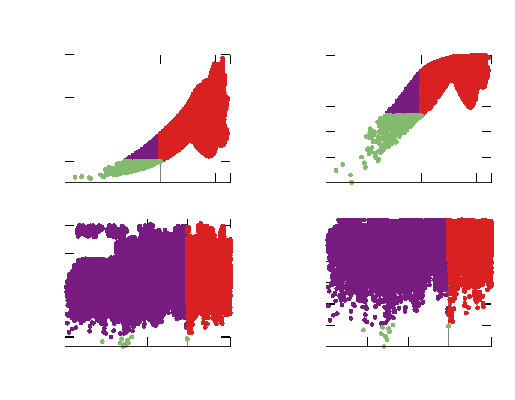
\includegraphics{./figures/h_and_h_not_fig}}%
    \gplfronttext
  \end{picture}%
\endgroup

  \vspace{0.3cm}
  \caption{\small The $\psi$-field (left) and \texttt{r}-field (right) of a
           configuration where Observation \ref{obs:observation_o} may (top)
           and may not (bottom) be made for $\delta \leq \delta_0$. Bottom:
           in contrast to the top row, set $\mathcal{V}$ is empty of admissible
           pose estimates for $\delta < 4.5 \ (\text{m}^2 +
           \text{rad}^2)^{1/2}$. The effect is produced in environment
           WILLOWGARAGE (pose $\bm{p}_{i}^G$; subsection \ref{subsec:exp_b})
           due to (a) the repetition of the immediate environment of the sensor
           more than once in the given map, and (b) the non-panoramic angular
           range of the sensor}
  \vspace{-0.5cm}
  \label{fig:h_and_h_not_fig}
\end{figure}


%%%%%%%%%%%%%%%%%%%%%%%%%%%%%%%%%%%%%%%%%%%%%%%%%%%%%%%%%%%%%%%%%%%%%%%%%%%%%%%%
%%%%%%%%%%%%%%%%%%%%%%%%%%%%%%%%%%%%%%%%%%%%%%%%%%%%%%%%%%%%%%%%%%%%%%%%%%%%%%%%
\subsection{The CBGL System}

In the same vein as Hypothesis \ref{hpt:hypothesis_h} assume the \texttt{r}-field
$f_{\texttt{r}}^{\bm{M}}(\mathcal{H})$ corresponding to the $\psi$-field
$f_{\psi}^{\bm{M}}(\mathcal{H})$ on a given map $\bm{M}$ (Def.
\ref{def:definition_5}) such that $\Psi[\texttt{I}^{\ast}] = \Psi_\uparrow$,
and $f_{\texttt{r}}^{\bm{M}}(\mathcal{H}[\texttt{I}^{\ast}]) = \texttt{I}$.
Then the top $k \ll |\mathcal{H}|$ ranked pose hypotheses
$\mathcal{H}[\texttt{I}^{\ast}]_{0:k-1}$ define set $\mathcal{V}$ such that
$\psi_0 = \max f_{\psi}^{\bm{M}}(\mathcal{H}[\texttt{I}^{\ast}]_{0:k-1})$,
and for all $\hat{\bm{p}}_\mathcal{V} \in \mathcal{V}$
and any $\hat{\bm{p}}_{\mathcal{X}} \in \mathcal{X}$:
$ f_{\texttt{r}}^{\bm{M}}(\hat{\bm{p}}_\mathcal{V}) < f_{\texttt{r}}^{\bm{M}}(\hat{\bm{p}}_{\mathcal{X}}) \Leftrightarrow
f_{\psi}^{\bm{M}}(\hat{\bm{p}}_\mathcal{V}) < f_{\psi}^{\bm{M}}(\hat{\bm{p}}_\mathcal{X}) \Leftrightarrow
\|\bm{p}-\hat{\bm{p}}_\mathcal{V}\|_2 < \|\bm{p}-\hat{\bm{p}}_{\mathcal{X}}\|_2$.
By identifying the pose estimates that correspond to the bottom $k$ CAER
values, this rationale attempts to recover the identity of the pose hypotheses
with the bottom $k$ pose errors across $\mathcal{H}$. It constitutes the core
of the proposed passive global localisation method, termed CBGL, and is
described in block diagram form in figure \ref{fig:block_system} (right) and in
pseudocode in Algorithm
%\ref{alg:bottom_k}
II \cite{Filotheou2023c}.

Assuming the satisfaction of Observation \ref{obs:observation_o}, the challenge
is choosing such $k$, $d_{\bm{l}}$, and $d_\alpha$ that, given pose estimate
error requirements $\delta_{\bm{l}}$, $\delta_{\theta}$ (Def.
\ref{def:definition_7}; Hyp.  \ref{hpt:hypothesis_h}), CBGL produces admissible
pose estimates while being executed in timely manner.  Given the rank field's
Monte Carlo nature, optimistically, the only option for increasing the accuracy
of the final pose estimate by a factor of two is doubling the densities of the
\texttt{r}-field; instead of doing that---and thereby doubling the method's
execution time---subsequent to the estimation of the pose estimates with the
$k$ lowest CAER values, CBGL utilises scan--to--map-scan matching
\cite{Vasiljevic2016c,Filotheou2023a}, followed by the estimation of the one
pose estimate with the lowest CAER value within the group of $k$ matched
estimates.
Matching allows for (a) the correction of the pose of true positive estimates
by scan-matching the map-scan captured from a pose estimate against the range
scan measured by the real sensor, (b) by the same token the potential
divergence of spurious, false positive, pose estimates, and hence their
elimination as pose estimate candidates, (c) the production of finer pose
estimates without excessive increase in execution time, and (d) the decoupling
of the final pose estimate's error from the field's densities.
%Selecting among all matched estimates the one with the minimum CAER allows for
%the system's delivery of one pose estimate response.
Figure \ref{fig:block_system} (left) and Algorithm
%\ref{alg:cbgl}
I \cite{Filotheou2023c} present the proposed method of CBGL in block diagram and
algorithmic forms respectively.

\begin{figure}\vspace{-0.4cm}
  \subfloat{\label{fig:cbgl}     \input{./figures/cbgl_system_tiny.tikz}}
  \subfloat{\label{fig:bottom_k} \input{./figures/inner_ranking_system2_tiny.tikz}}
  \caption{\small CBGL in block diagram form. Left: Given a LIDAR's 2D
           measurement $\mathcal{S}_R$ and a map $\bm{M}$, CBGL generates a set
           of pose hypotheses $\mathcal{H}$ and estimates the $k$ hypotheses
           with the least pose error (right; alg.
           %\ref{alg:bottom_k}
           II \cite{Filotheou2023c}). Then it scan--to--map-scan matches those
           to $\mathcal{S}_R$ for finer estimation (\texttt{sm2}; alg.
           %\ref{alg:sm2}
           III \cite{Filotheou2023c}). CBGL's output pose estimate is
           that with the least CAER among the $k$ matched estimates.  Right:
           CBGL's core method. Given $\mathcal{S}_R$, $\bm{M}$, and pose
           estimates $\mathcal{P}$, it (a) computes and ranks the CAER values
           between $\mathcal{S}_R$ and map-scans captured from $\mathcal{P}$
           within $\bm{M}$, and (b) outputs the hypotheses with the $k$ lowest
           CAER values}
\vspace{-0.5cm}
  \label{fig:block_system}
\end{figure}


%%% CBGL %%%%%%%%%%%%%%%%%%%%%%%%%%%%%%%%%%%%%%%%%%%%%%%%%%%%%%%%%%%%%%%%%%%%%%%%
%\floatstyle{spaceruled}
%\restylefloat{algorithm}
%\begin{algorithm}[]
  %\caption{\texttt{CBGL}}
  %\begin{spacing}{1.0}
  %\begin{algorithmic}[1]
    %\REQUIRE $\mathcal{S}_R$, $\bm{M}$, $(d_{\bm{l}}, d_\alpha)$, $k$
    %\ENSURE Pose estimate of sensor measuring range scan $\mathcal{S}_R$ %$\hat{\bm{p}}$
    %\STATE $A \leftarrow \texttt{calculate\_area}(\texttt{free}(\bm{M}))$
    %\STATE $\mathcal{H} \leftarrow \{\varnothing\}$
    %\FOR {$i \leftarrow 0,1,\dots,d_{\bm{l}} \cdot A-1$}
      %\STATE \small $(\hat{x},\hat{y},\hat{\theta}) \leftarrow \texttt{rand()}$: $(x,y) \in \texttt{free}(\bm{M})$, $\hat{\theta} \in [-\pi,+\pi)$
      %\FOR {$j \leftarrow 0,1,\dots, d_{\alpha}-1$}
        %\STATE $\mathcal{H} \leftarrow \{\mathcal{H}, (\hat{x}, \hat{y}, \hat{\theta} + j \cdot 2\pi / d_{\alpha})\}$     \label{alg:cbgl:h}
      %\ENDFOR
    %\ENDFOR
    %\STATE $\mathcal{H}_1 \leftarrow$ \texttt{bottom}$\_k\_\texttt{poses}(\mathcal{S}_R, \bm{M}, \mathcal{H}, k)$ \hfill {\small (Alg. \ref{alg:bottom_k}}) \label{alg:cbgl:h1}
    %\STATE $\mathcal{H}_2 \leftarrow \{\varnothing \}$
    %\FOR {$k \leftarrow 0,1,\dots,|\mathcal{H}_1|-1$}
      %\STATE $\hat{\bm{h}}^\prime \leftarrow \texttt{sm2}(\mathcal{S}_R, \bm{M}, \mathcal{H}_1[k])$ \hfill {\small (Alg. \ref{alg:sm2} or e.g. \texttt{x1} \cite{Filotheou2023a}})
      %\STATE $\mathcal{H}_2 \leftarrow \{\mathcal{H}_2, \hat{\bm{h}}^\prime\}$  \label{alg:cbgl:h2}
    %\ENDFOR
    %\RETURN \texttt{bottom}$\_k\_\texttt{poses}(\mathcal{S}_R, \bm{M}, \mathcal{H}_2, 1)$
  %\end{algorithmic}
  %\end{spacing}
  %\label{alg:cbgl}
%\end{algorithm}

%%% Bottom-n %%%%%%%%%%%%%%%%%%%%%%%%%%%%%%%%%%%%%%%%%%%%%%%%%%%%%%%%%%%%%%%%%%%%
%\floatstyle{spaceruled}
%\restylefloat{algorithm}
%\begin{algorithm}[]
  %\caption{\texttt{bottom}\_$k$\_\texttt{poses}}
  %\begin{spacing}{1.0}
  %\begin{algorithmic}[1]
    %\REQUIRE $\mathcal{S}_R$, $\bm{M}$, $\mathcal{H}$, $k$
    %\ENSURE $\mathcal{H}_{\triangledown}$
    %\STATE $\Psi \leftarrow \{\varnothing \}$
    %\FOR {$h \leftarrow 0,1,\dots,|\mathcal{H}|-1$}
      %\STATE $\mathcal{S}_V^{\hspace{1pt} h} \leftarrow \texttt{scan\_map}(\bm{M}, \mathcal{H}[h])$
      %\STATE $\psi \leftarrow 0$
      %\FOR {$n \leftarrow 0,1,\dots,|\mathcal{S}_R|-1$}
        %\STATE $\psi \leftarrow \psi + \big|\mathcal{S}_R[n]-\mathcal{S}_V^{\hspace{1pt} h}[n]\big|$ \hfill {\small (Eq. (\ref{eq:caer})})
      %\ENDFOR
      %\STATE $\Psi \leftarrow \{\Psi, \psi\}$
    %\ENDFOR
    %\STATE $[\Psi_{\uparrow}, \texttt{I}^{\ast}] \leftarrow \texttt{sort}(\Psi, \texttt{asc})$
    %\STATE $\mathcal{H}_{\triangledown} \leftarrow \{\varnothing \}$
    %\FOR {$h \leftarrow 0,1,\dots,k-1$}
      %\STATE $\mathcal{H}_{\triangledown} \leftarrow \{\mathcal{H}_{\triangledown}, \mathcal{H}[\texttt{I}^{\ast}[h]]\}$
    %\ENDFOR
    %\RETURN $\mathcal{H}_{\triangledown}$
  %\end{algorithmic}
  %\end{spacing}
  %\label{alg:bottom_k}
%\end{algorithm}

%%% sm2 %%%%%%%%%%%%%%%%%%%%%%%%%%%%%%%%%%%%%%%%%%%%%%%%%%%%%%%%%%%%%%%%%%%%%%%%%
%\floatstyle{spaceruled}
%\restylefloat{algorithm}
%\begin{algorithm}[]
  %\caption{\texttt{sm2}}
  %\begin{spacing}{1.0}
  %\begin{algorithmic}[1]
    %\REQUIRE $\mathcal{S}_R$, $\bm{M}$, $\hat{\bm{p}}$
    %%\ENSURE $\hat{\bm{p}}^\prime$
    %\ENSURE $\hat{\bm{p}}$ $+$ correction that aligns $\mathcal{S}_V^{\bm{M}}(\hat{\bm{p}})$ to $\mathcal{S}_R$
    %\STATE $\mathcal{S}_V \leftarrow \texttt{scan\_map}(\bm{M}, \hat{\bm{p}})$
    %\STATE $\bm{\Delta p} \leftarrow \texttt{scan-match}(\mathcal{S}_R,\mathcal{S}_V)$ \hfill {\small (e.g. \texttt{ICP}\cite{Vizzo2023}, \texttt{FSM}\cite{Filotheou2022f}})
    %%\STATE $\hat{\bm{p}}^\prime \leftarrow \hat{\bm{p}} + \bm{\Delta p}$
    %%\RETURN $\hat{\bm{p}}^\prime$
    %\RETURN $\hat{\bm{p}} + \bm{\Delta p}$
  %\end{algorithmic}
  %\end{spacing}
  %\label{alg:sm2}
%\end{algorithm}
